% Author: Dun-Ming Huang
% Email: dunmingbrandonhuang@berkeley.edu
% CSM16A Spring 2023
\qns{A Trace on the Projections of Vectors and Its Techniques}

\textbf{Learning Goal: }
\begin{bindenum}
    \item Learn the defining features of a vector projection via part-by-part derivations
    \item Explore the extension of projection as an in-course concept via (1) looking at projection of vectors onto different geometries and (2) exploring the application of projection on linear algebra/geometry problems.
\end{bindenum}

\begin{enumerate}
    \item {
        Suppose we have the following vectors, $\vec{v}, \vec{v}^* \in \R^2$:
        \begin{center}
            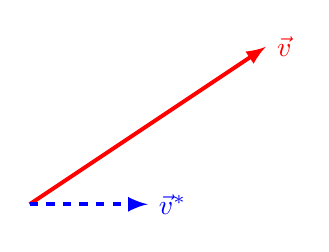
\begin{tikzpicture}[>=latex]
              \draw[->,line width=0.5mm, red] (0,0) -- (3,2) node[right]{$\vec{v}$};
              \draw[dashed, ->, line width=0.5mm, blue] (0,0) -- (1.5,0) node[right]{$\vec{v}^*$};
            \end{tikzpicture}
        \end{center}
        where $\vec{v}^*$ has a zero second component and a nonzero first component.
        If $\vec{v}$ is a linear combination of $\vec{v}^*$ and another vector perpendicular to $\vec{v}^*$, then what is the coefficient of $\vec{v}^*$ in this linear combination in terms of $\vec{v}$ and $\vec{v}^*$?
        
    }
    \meta { 
        Here, instructor can let \textbf{students present the primarily described solution, then have mentors bring in the cosine perspective}. This order of introduction will allow students to utilize the cosine insight in subpart (b). \\
        \textbf{Students are not expected to suddenly learn why the cosine identity is useful}. Projection is one of the linear algebra concepts that \textbf{let students learn why cosine is useful}.
        
    }
    \ans { 
        We may notice that $\vec{v}^*$ is some vector along the x-axis, and therefore may be expressed as something to the effect of:
        \[
            \vec{v}^* = \begin{bmatrix} v_1^* \\ 0 \end{bmatrix}
        \]
        Meanwhile, we know that the vector $\vec{v}$ can be computed as its components:
        \[
            \vec{v} = \begin{bmatrix} v_1 \\ v_2 \end{bmatrix} = \frac{v_1}{v_1^*} \begin{bmatrix} v_1^* \\ 0 \end{bmatrix} + v_2 \begin{bmatrix} 0 \\ 1 \end{bmatrix}
        \]
        Therefore, the coefficient of $\vec{v}^*$ in this linear combination of the prompt would be: $\frac{v_1}{v_1^*}$.
        \par
        We can recognize that such value originates from the cosine of angle between $\vec{v}$ and $\vec{v}^*$:
        \begin{center}
            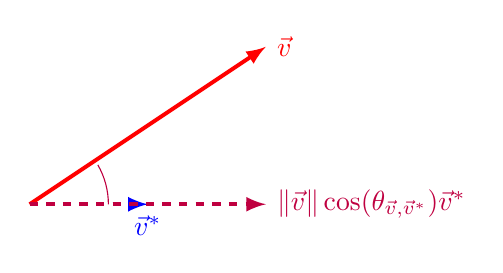
\begin{tikzpicture}[>=latex]
              \draw[->,line width=0.5mm, red] (0,0) -- (3,2) node[right]{$\vec{v}$};
              \draw[dashed, ->, line width=0.5mm, blue] (0,0) -- (1.5,0) node[below]{$\vec{v}^*$};
              \draw[dashed, ->, line width=0.5mm, purple] (0,0) -- (3,0) node[right]{$\| \vec{v} \| \cos(\theta_{\vec{v}, \vec{v}^*}) \vec{v}^*$};
              \draw[purple] (1, 0) arc (0:30:1);
            \end{tikzpicture}
        \end{center}
        where, we may obtain from cosine law (the derivation is not shown here, but you may ask your mentor to supply it) that:
        \[
            \cos(\theta_{\vec{v}, \vec{v}^*}) =
            \frac{\vec{v} \cdot \vec{v}^*}{\| \vec{v} \| \| \vec{v}^* \|}
        \]
        Using cosine has another significance: the linear combination of $\vec{v}$ now becomes the sum of a scaled $\vec{v}^*$ and some vector perpendicular to it, as the prompt requires. \\
        Then, we obtain that the magnitude of the linear combination component with $\vec{v}^*$ is:
        \[
            \| \vec{v} \| \cos(\theta_{\vec{v}, \vec{v}^*}) = \frac{\vec{v} \cdot \vec{v}^*}{\| \vec{v}^* \|}
        \]
        and we multiply such magnitude by the unit vector in direction of $\vec{v}^*$, such that we have the component of $\vec{v}$'s linear combination that lies on the direction of $\vec{v}^*$. \\
        For why we need the unit vector in direction of $\vec{v}^*$, it is because multiplying a unit vector by any scalar $\alpha$ makes that product have a magnitude of $\alpha$, and we multiply $\frac{\vec{v}^*}{\|\vec{v}^*\|}$ by the magnitude of its corresponding component in $\vec{v}$ to obtain the exact component for our linear combination:
        \[
            \frac{\vec{v}^*}{\|\vec{v}^*\|} \| \vec{v} \| \cos(\theta_{\vec{v}, \vec{v}^*})
            = \frac{\vec{v} \cdot \vec{v}^*}{{\| \vec{v}^* \|}^2} \vec{v}^*
        \]
        and to verify this coefficient on part (a),
        \[
            \frac{\vec{v} \cdot \vec{v}^*}{{\| \vec{v}^* \|}^2} = \frac{v_1 v_1^*}{{v_1^*}^2} = \frac{v_1}{v_1^*}
        \]
        
    }
    \item {
        Suppose we have the following vectors, $\vec{w}, \vec{w}' \in \R^2$:
        \begin{center}
            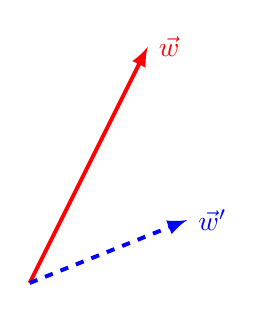
\begin{tikzpicture}[>=latex]
              \draw[->,line width=0.5mm, red] (0,0) -- (1.5,3) node[right]{$\vec{w}$};
              \draw[dashed, ->, line width=0.5mm, blue] (0,0) -- (2,0.8) node[right]{$\vec{w}'$};
            \end{tikzpicture}
        \end{center}
        If $\vec{w}$ is a linear combination of $\vec{w}'$ and another vector perpendicular to $\vec{w}'$, then what is the coefficient of $\vec{w}'$ in this linear combination? 
        
    }
    \meta { 
        A more complicated explanation may utilize a rotated coordinate system, where the blue (and purple) vectors are the new ``x-axis''; however, this is not more intuitive than the explanation offered in part (a). 
        
    }
    \ans { 
        I will reuse the logic illustrated in previous part's solution to state the coefficient as:
        \[
            \frac{\vec{w} \cdot \vec{w}'}{{\| \vec{w}' \|}^2}
        \]
    }
    \item {
        To defend your answers in part (b), suppose the solution you have in $b$ can be expressed as a variable $x^*$, prove the following statement:
        \begin{quote}
            Such solution $x^*$ presents the smallest possible value for the expression $\| \vec{w} - x \vec{w}' \|$, where $x \in \R$.
        \end{quote}
        
    }
    \meta { 
        There are a couple of general ways to prove this problem:
        \begin{itemize}
            \item Use \textbf{Pythagorean Theorem to show} that choosing any other scalar multiple of $\vec{w}'$ does not provide a smaller difference.
            \item Directly use calculus to minimize the expression.
        \end{itemize}
        \textbf{Numerically, the latter option is much easier to express.} \\
        The Pythagorean approach is briefly outlined as:
        \begin{itemize}
            \item Suppose there exists another choice of $x$, $x'$, that allows for a smaller norm $\| \vec{w} - x \vec{w}'\|$.
            \item Then, use Pythagorean Theorem to show that the new choice of $x'$ causes a right triangle where the hypotenuse is $\vec{w} - x' \vec{w}'$, and the shorter sides are $x^*\vec{w}' - x'\vec{w}'$ and $\vec{w} - x^* \vec{w}'$
        \end{itemize}
        
    }
    \ans { 
        We may first notice that the vector $\vec{w} - x^* \vec{w}'$ is perpendicular to $\vec{w}'$ due to part (b)'s prompt requirement. \\
        Now, let us see what is the smallest possible value for the expression $\| \vec{w} - x \vec{w}'\|$, which is the norm of a vector and therefore must be nonnegative. In this case, since this number if either zero or positive, minimizing this number is equivalent to minimizing its squared version.
        \par
        For convenience, we would also like to minimize its squared version than its original. \\
        Observe that,
        \[
            \begin{cases}
                \| \vec{w} - x \vec{w}'\| &= \sqrt{ {(\vec{w} - x \vec{w}')}^T {(\vec{w} - x \vec{w}')} } \\
                {\| \vec{w} - x \vec{w}'\|}^2 &= {(\vec{w} - x \vec{w}')}^T {(\vec{w} - x \vec{w}')}
            \end{cases}
        \]
        not having the square root is a tad more convenient for the mathematical writing (for both you and I), and we would only have to square-root the resulting minimization of a squared variable to gain the variable's true minimal value.
        \par
        Now, let us attempt to find a lowerbound for our expression of prompt:
        \begin{align*}
            {\| \vec{w} - x \vec{w}'\|}^2 &= {(\vec{w} - x \vec{w}')}^T {(\vec{w} - x \vec{w}')} \\
            &= \vec{w}^T \vec{w} - 2 x \vec{w} \cdot \vec{w}' + x^2 \vec{w}^{'^T} \vec{w}'
        \end{align*}
        Notice that to minimize the above expression, we can take its derivative with respect to $x$, and since the above expression is a quadratic function with positive coefficient for second-order term, its second-order derivative will be positive and cause the function to have one distinct minimum:
        \begin{align*}
            \frac{\rm d}{\rm dx} \vec{w}^T \vec{w} - 2 x \vec{w} \cdot \vec{w}' + x^2 \vec{w}^{'^T} \vec{w}'
            &= 2 (\vec{w}^{'^T} \vec{w}' x - \vec{w} \cdot \vec{w}') \\
            2 (\vec{w}^{'^T} \vec{w}' x_{\min} - \vec{w} \cdot \vec{w}') &= 0 \\
            x_{\min} &= \frac{\vec{w} \cdot \vec{w}'}{\vec{w}^{'^T} \vec{w}'}
        \end{align*}
        We observe that the minimizing $x_{\min}$ for the expression ${\| \vec{w} - x \vec{w}'\|}^2$ is exactly as we found in part (b). \\
        Furthermore, because $x_{\min}$ minimizes the square of a \textbf{nonnegative} variable $\| \vec{w} - x \vec{w}'\|$, it minimizes its original version as well, because no other possible real $x$ can minimize its squared version further than $x_{\min}$ has \textit{(Here, nonnegative is the crucial factor of such observation)}.
        
    }
\end{enumerate}
Up to here, we have unlocked a mathematical operation between vectors called ``projection'', defined along your solutions as follows:
\begin{ln-define}{Projection of Vectors}{}
    The projection of a vector $\vec{x}$ onto $\vec{w}$ is the vector in the direction of $\vec{w}$ (or, is a scalar multiple of $\vec{w}$) that has the magnitude of:
    \[
        \| {proj}_{\vec{w}} (\vec{x}) \| = \frac{\vec{w} \cdot \vec{x}}{\|\vec{w}\|}
    \]
    and is the closest vector to $\vec{x}$ along the direction of $\vec{w}$.
\end{ln-define}
% \begin{enumerate}[resume]
%     \item {
%         Now, instead of projecting vectors onto another vector, I will project vectors onto a span of vectors:
%         \[
%             \mathcal{S} = span \bigg\{
%                 \begin{bmatrix} 1 \\ 2 \\ 0 \end{bmatrix},
%                 \begin{bmatrix} 1 \\ 0 \\ 0 \end{bmatrix}
%             \bigg\}
%         \]
%         Don't worry about the curvy $\mathcal{S}$, it's here for aesthetics and can be treated as just the letter $S$. \\
%         Then propose a method of finding:
%         \[
%             {proj}_{\mathcal{S}} \bigg( \begin{bmatrix} 2 \\ 2 \\ 3 \end{bmatrix} \bigg)
%         \]
%         to your classmates and mentor, and discuss whether this approach does recover the projection. \\
%         \textit{Hint: the projection of a vector $\vec{v}$ onto a span is the closest vector to $\vec{v}$ that exists on such span. Looking back at part (a) and part (b)'s conditions of a projection, what does it say about the relationship between the span and the difference between $\vec{v}$ and projection?}
        
%     }
%     \meta {
%         This problem tests the skill of observing a problem. In particular, here are some hints you can offer your mentors:
%         \begin{enumerate}
%             \item What is the property of a projection?
%             \item What is the property of a projection direction and the vector-projection subtraction difference?
%             \item How do we solve for the projection itself, and what does it lie on (exist at)?
%             \item How do we solve linear systems of equations?
%         \end{enumerate}
%         You may also notice that this is a \textbf{soft introduction to least squares} algorithm.

%     }
%     \ans {
%         Let us begin our analysis with a visualization:
%         \begin{center}
%             \begin{tikzpicture}[>=latex, axis/.style={->,black,thick},]
%                 \draw[axis] (0,0,0) -- (4,0,0) node[anchor=north east]{$x$};
%                 \draw[axis] (0,0,0) -- (0,4,0) node[anchor=north west]{$z$};
%                 \draw[axis] (0,0,0) -- (0,0,4) node[anchor=south]{$y$};
%                 \draw[dashed, ->,line width=0.5mm] (0, 0, 0) -- (2, 3, 2) node[right]{$\begin{bmatrix} 2 \\ 2 \\ 3 \end{bmatrix}$};
%                 \draw[dashed, ->,line width=0.5mm, red] (0, 0, 0) -- (1, 0, 2) node[right]{$\begin{bmatrix} 1 \\ 2 \\ 0 \end{bmatrix}$};
%                 \draw[dashed, ->, line width=0.5mm, blue] (0, 0, 0) -- (1, 0, 0) node[right]{$\begin{bmatrix} 1 \\ 0 \\ 0 \end{bmatrix}$};
%             \end{tikzpicture}
%         \end{center}
%         The definition of projection states that it must be the closest vector to $\begin{bmatrix} 2 \\ 2 \\ 3 \end{bmatrix}$ on the span $\mathcal{S}$. \\
%         Therefore, the difference between our vector and its difference must be orthogonal (perpendicular) to the span $\mathcal{S}$. \\
%         In other words, we solve the following systems of equation, such that suppose $\vec{v}$ is the projection the prompt desires:
%         \[
%             \begin{cases}
%                 { \bigg(\begin{bmatrix} 2 \\ 2 \\ 3 \end{bmatrix} - \vec{v}\bigg) }^T \begin{bmatrix} 1 \\ 2 \\ 0 \end{bmatrix} = 0 \\
%                 { \bigg(\begin{bmatrix} 2 \\ 2 \\ 3 \end{bmatrix} - \vec{v}\bigg) }^T \begin{bmatrix} 1 \\ 0 \\ 0 \end{bmatrix} = 0 \\
%             \end{cases}
%         \]
%         Recognize that because $\vec{v}$ exists on the span $\mathcal{S}$, there exists some vector $\vec{x}$ such that:
%         \[
%             \vec{v} = \begin{bmatrix}
%                 1 & 1 \\
%                 2 & 0 \\
%                 0 & 0
%             \end{bmatrix} \vec{x} =
%             x_1 \begin{bmatrix} 1 \\ 2 \\ 0 \end{bmatrix} + x_2 \begin{bmatrix} 1 \\ 0 \\ 0 \end{bmatrix}
%         \]
%         We may rephrase this system of equation in the form of matrix-vector multiplications:
%         \begin{align*}
%             \begin{bmatrix}
%                 1 & 2 & 0 \\
%                 1 & 0 & 0
%             \end{bmatrix}
%             (\begin{bmatrix} 2 \\ 2 \\ 3 \end{bmatrix} - \vec{v}) &= \vec{0} \\
%             \begin{bmatrix}
%                 1 & 2 & 0 \\
%                 1 & 0 & 0
%             \end{bmatrix}
%             \begin{bmatrix} 2 \\ 2 \\ 3 \end{bmatrix} &= 
%             \begin{bmatrix}
%                 1 & 2 & 0 \\
%                 1 & 0 & 0
%             \end{bmatrix}
%             \begin{bmatrix}
%                 1 & 1 \\
%                 2 & 0 \\
%                 0 & 0
%             \end{bmatrix} \vec{x} \\
%             \vec{x} &= {\bigg( \begin{bmatrix}
%                 1 & 2 & 0 \\
%                 1 & 0 & 0
%             \end{bmatrix}
%             \begin{bmatrix}
%                 1 & 1 \\
%                 2 & 0 \\
%                 0 & 0
%             \end{bmatrix} \bigg)}^{-1}
%             \begin{bmatrix}
%                 1 & 2 & 0 \\
%                 1 & 0 & 0
%             \end{bmatrix}
%             \begin{bmatrix} 2 \\ 2 \\ 3 \end{bmatrix}
%         \end{align*}
%         In the end, we may compute that:
%         \begin{align*}
%             \vec{x} &=
%             {\bigg( \begin{bmatrix}
%                 1 & 2 & 0 \\
%                 1 & 0 & 0
%             \end{bmatrix}
%             \begin{bmatrix}
%                 1 & 1 \\
%                 2 & 0 \\
%                 0 & 0
%             \end{bmatrix} \bigg)}^{-1}
%             \begin{bmatrix}
%                 1 & 2 & 0 \\
%                 1 & 0 & 0
%             \end{bmatrix}
%             \begin{bmatrix} 2 \\ 2 \\ 3 \end{bmatrix} \\
%             &= \frac{1}{4} \begin{bmatrix} 1 & -1 \\ -1 & 5 \end{bmatrix}
%             \begin{bmatrix} 6 \\ 2 \end{bmatrix}
%             = \begin{bmatrix} 1 \\ 1 \end{bmatrix} \\
%             \vec{v} &= A \vec{x} \\
%             &= \vec{v} = \begin{bmatrix}
%                 1 & 1 \\
%                 2 & 0 \\
%                 0 & 0
%             \end{bmatrix} \begin{bmatrix} 1 \\ 1 \end{bmatrix}
%             = \begin{bmatrix} 2 \\ 2 \\ 0 \end{bmatrix}
%         \end{align*}
%         such vector is therefore the projection we look for.
    
%     }
% \end{enumerate}
% Via the observations above, we may later generalize that,
% \begin{ln-define}{Projection of Vectors onto Vector Spaces}{}
%     The projection of a vector $\vec{x}$ onto $\mathcal{S} = span \{\vec{w}_1, \dots, \vec{w}_n\}$ is the vector in the span of $\{\vec{w}_1, \dots, \vec{w}_n\}$ (or, also belongs to such span) such that:
%     \begin{align*}
%         W &= \begin{bmatrix} \vec{w}_1 & \cdots & \vec{w}_n \end{bmatrix} \\
%         proj_{\mathcal{S}} (\vec{x}) &= W {(W^T W)}^{-1} W^T \vec{x}
%     \end{align*}
% \end{ln-define}
% Now, let us explore an application of projection slightly beyond the scope of lectures:
% \begin{enumerate}[resume]
%     \item {
%         Suppose that I have the following line:
%         \[
%             2x + 5y = 0
%         \]
%         Find the closest distance between this line and the point $(5, 2)$.
        
%     }
%     \meta { 
%         Encourage students to observe the problem:
%         \begin{enumerate}
%             \item How do we, in general, find the shortest distance?
%             \item Once we have decided on the above, how is this problem representable in a vector perspective?
%             \item Furthermore, what are parts of the problem that is related to projection and its property? Remember that projection of $\vec{x}$ onto $\vec{w}$ is the closest vector to $\vec{x}$ that is in the direction of $\vec{w}$.
%         \end{enumerate}
        
%     }
%     \ans { 
%         To find the distance between a point and a line is to find the difference between the vector that can represent that line and the point of question. \\
%         Suppose that we represent the line $2x + 5y = 0$ in terms of vectors:
%         \[
%             \begin{bmatrix} 2 \\ 5 \end{bmatrix}^T \begin{bmatrix} x \\ y \end{bmatrix} = 0
%         \]
%         such that the line is in fact a set of vectors:
%         \[
%             \mathcal{L} = \bigg\{
%                 \begin{bmatrix} x \\ y \end{bmatrix} |
%                 \begin{bmatrix} 2 \\ 5 \end{bmatrix}^T \begin{bmatrix} x \\ y \end{bmatrix} = 0
%             \bigg\}
%         \]
%         We will also find that the vector $\begin{bmatrix} 2 \\ 5 \end{bmatrix}$ is perpendicular to any other vector belonging to $\mathcal{L}$ (because their dot product is $0$). Therefore, my shortest distance can be expressed as the magnitude of a scaled version of $\begin{bmatrix} 2 \\ 5 \end{bmatrix}$. Let's abbreviate this vector as $\vec{w}$ from now on for convenience.
%         \par
%         The shortest distance between a point and a line ought to be perpendicular to the line itself. We may then observe that, suppose $\vec{X}$ is the projection of the vector of point $(5, 2)$ onto the line, their differences is also parallel to the vector of $\begin{bmatrix} 2 \\ 5 \end{bmatrix}$, perpendicular to the line. Therefore, there exists some constant $\alpha$ such that
%         \begin{align*}
%             \begin{bmatrix} 5 \\ 2 \end{bmatrix} - \vec{X}
%             &= \alpha \begin{bmatrix} 2 \\ 5 \end{bmatrix} \\
%             \bigg( \begin{bmatrix} 5 \\ 2 \end{bmatrix} - \vec{X} \bigg)
%             \cdot \begin{bmatrix} 2 \\ 5 \end{bmatrix}
%             &= \alpha \begin{bmatrix} 2 \\ 5 \end{bmatrix} \cdot \begin{bmatrix} 2 \\ 5 \end{bmatrix} \\
%             20 &= \alpha \cdot 29 \\
%             \alpha &= \frac{20}{29}
%         \end{align*}
%         Therefore, the shortest distance between the point and line of question would be:
%         \[
%             \|\alpha \begin{bmatrix} 2 \\ 5 \end{bmatrix}\| = |\alpha| \sqrt{29} = \frac{20}{29} \sqrt{29}
%         \]
        
%     }
%     \item {
%         Suppose instead that I have the following set of vectors:
%         \[
%             \mathcal{H} = \{
%                 \vec{x} | \vec{w} \cdot \vec{x} + 4 = 0
%             \}
%         \]
%         where $\vec{w}$ is orthogonal to any vector in $\mathcal{H}$.
%         Find the closest distance between this set of vectors and the point $(10, 11, 2)$ in terms of $\vec{w}$.
        
%     }
%     \meta { 
%         This problem is a case of application for students to practice the techniques of part (e) on a slightly different setting.
        
%     }
%     \ans { 
%         We will employ the same logic from part (e), which is to suppose that:
%         \begin{quote}
%             Let $\vec{x}$ represent the point $(10, 11, 2)$, and $\vec{y}$ be the orthogonal vector to $\mathcal{H}$ that is the difference between $\vec{x}$ and ${proj}_{\mathcal{H}}(\vec{x})$. Then, such difference should also be a multiple of $\vec{w}$ as well, which is orthogonal to $\mathcal{H}$, such that:
%             \[
%                 (\vec{x} - \vec{y}) = \alpha \vec{w}
%             \]
%         \end{quote}
%         Therefore, the arithmetic follows:
%         \begin{align*}
%             (\vec{x} - \vec{y}) &= \alpha \vec{w} \\
%             (\vec{x} - \vec{y}) \cdot \vec{w} &= \alpha \vec{w} \cdot \vec{w} \\
%             \vec{y} \in \mathcal{H} &\implies \vec{y} \cdot \vec{w} + 4 = 0 \\
%             \begin{bmatrix} 10 \\ 11 \\ 2 \end{bmatrix} \cdot \vec{w} + 4 &= \alpha \vec{w} \cdot \vec{w} \\
%             \alpha &= \frac{\begin{bmatrix} 10 & 11 & 2 \end{bmatrix} \vec{w} + 4}{\vec{w} \cdot \vec{w}}
%         \end{align*}
%         Then, the shortest distance between $(10, 11, 2)$ and $\mathcal{H}$ may be expressed as:
%         \[
%             \frac{\begin{bmatrix} 10 & 11 & 2 \end{bmatrix} \vec{w} + 4}{\vec{w} \cdot \vec{w}} \| \vec{w} \|
%         \]
        
%     }
%\end{enumerate}

